\documentclass[11pt]{article}
\usepackage[utf8]{inputenc}
\usepackage{booktabs}
\usepackage{multicol}
\usepackage{amsmath}
\usepackage{amsfonts}
\usepackage{fullpage}
\usepackage{amsmath,amssymb,amsthm}
\usepackage{tikz,lipsum,lmodern}
\usepackage[most]{tcolorbox}
\usepackage{graphicx}
\def\R{{\mathbb{R}}}
\def\N{{\mathbb{N}}}


\begin{center}
    
\includegraphics[width=17cm]{cover.png}
\end{center}

\newpage
\begin{document}
\section*{Abstract}
The purpose of the lab was to understand the absolute zero depending on the number of moles that are affecting the system. When keeping the number of moles constant, the apparatus was dumped into the water at different temperatures to determine the linear regression between the data points. From the constant moles, the linear trend from the experiment was $y=2.7x-190$, given that the absolute zero of the linear trend was $-190\pm 11^\circ$ Celsius when the pressure is equal to zero. Compared to the theoretical value of absolute zero ($-273^\circ$ Celsius), the error percentage obtained was $30\%$. \\
When fluctuating the number of moles, different varieties of a slope are obtained due to the ideal gas law equation; the more moles the system contains the less steep the temperature and pressure graph. From $0.043$ mols, the system had an absolute zero value of $-88\pm14^\circ$ Celsius when the apparatus went from hot, room-temperature, cold water. Then for $0.04$ mols, the system had an absolute zero value of $-130\pm15^\circ$ Celsius. For 0.06 mols, the absolute zero was $-100\pm2^\circ$ Celsius. All together, giving an average of $-110\pm26^\circ$ Celsius, which is an error percentage of $60\%$ compared to the theoretical value of absolute zero. Unfortunately, the experiment was not successful due to the high number of error percentages obtained. The errors can be explained by human errors, systematic errors, and the number of moles affecting the system. 

\section*{Introduction}
The purpose of the lab is to get an understanding of the absolute zero and how it is used. The Absolute Zero Apparatus is used to experimentally determine the temperature of absolute zero (in degrees Celsius). Absolute zero, by definition, is the point at which a gas exerts zero pressure. With a computer, the Absolute Zero Apparatus can help observing the relationship between temperature and pressure and use DataStudio to mathematically extrapolate to find absolute zero.\\
The Absolute Zero Apparatus consists of a Fast Response Temperature Sensor and plastic tubing (with pressure connector) mounted into a hollow copper sphere. When the sphere is submerged in a water bath and connected to a temperature sensor, pressure sensor, and a computer interface, Capstone records and displays the temperature and pressure.\\
For an ideal gas, the absolute pressure is directly propositional to the absolute temperature of the gas.
\begin{equation}
    T=\frac{PV}{nR}=\frac{N}{nR}P
\end{equation}
Thus a plot of temperature vs. pressure will result in a linear function.
\begin{equation}
    y=(slope)x+b
\end{equation}
Where the dependent value $y$ is the temperature, the independent value $x$ is the pressure, and the slope is the volume of moles and the gas constant. The slope of the linear function depends on the amount of gas in the thermometer, but regardless of the amount of gas, the intercept of the line with the temperature axis should be at absolute zero. If the plot measured temperature in Celsius, the intercept will not be zero, but rather the temperature of absolute zero in degrees Celsius.

\section*{Procedure}
Refer to "Absolute Zero Apparatus" instruction manual by PASCO. The experiment followed the exact basic set up and procedure as the manual. 

\section*{Data and Analysis}
The experiment's purpose is to familiarise with the concept of absolute zero when using ideal gas law (equation(1)). Keeping the number of moles and volume constant provides a pressure vs temperature graph, from which the y-intercept can be used to determine the temperature at zero pressure; in other words, absolute zero.\\
By keeping constant pressure, the volume containing the moles is being dunked under different water temperatures to collect a variety of data points. From the collective data points, the linear regression from the graphical analysis will provide a point at which the pressure will equate to zero. 
\begin{center}
    \textbf{Graph 1}: The Temperature According to Pressure in an Ideal Gas Law \\
    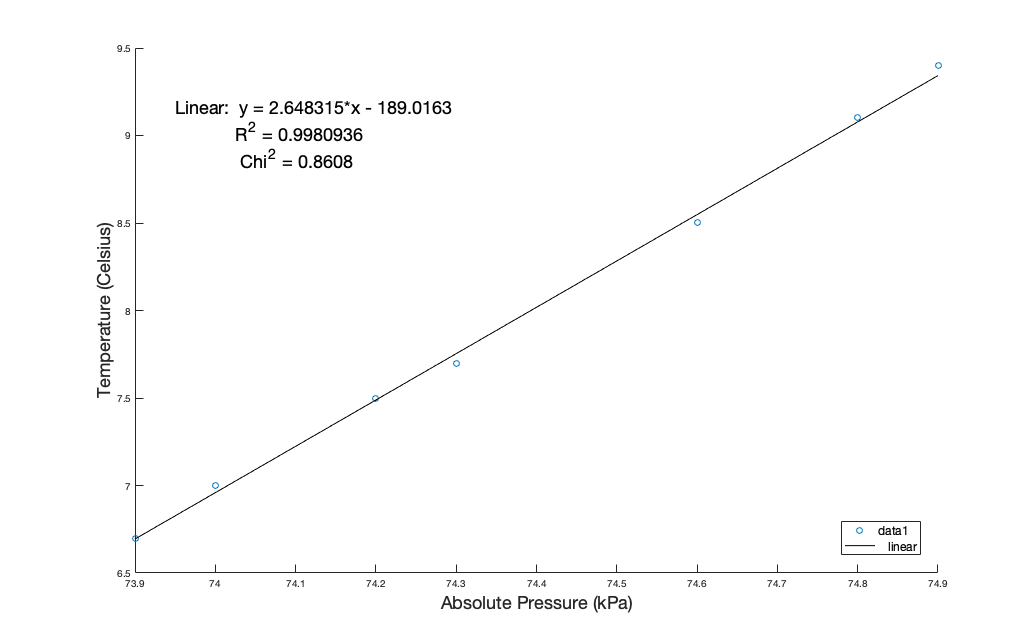
\includegraphics[width=16cm]{ex1.png}\\\textbf{Graph 1}: From the raw data collected from the absolute zero experiment, the independent value $x$ is the absolute pressure measured in kilopascals, and the dependent value $y$ is the temperature measured in Celsius. The blue scatter points are the data points collected from the experiment. The black linear regression has a function of $y=2.65x-189$ with the slope being $2.65\pm 0.14 \frac{\text{Celsius}}{kPa}$ with the y-intercept being $-189\pm 11 \text{ Celsius}$. Moreover, the $R^2$ value of the graph is $0.998$ indicates that the data is $99.8\%$ of the variation in the $y$ data is due to the variation in the $x$ data; giving a perfect slope of the alignment of the data. Furthermore, the Chi-squared value is $0.8608$, which implies that the model is accurately displayed to the actual observed data. 
\end{center}
Absolute zero contains zero pressure. According to the graph since the independent value $x$ is the absolute pressure. Then the y-intercept of the linear regression is considered to be the absolute zero point. From the collected information, the graph's slope is the volume of the container that contains the moles divided over the number of moles and the gas constant $R$, which follows equations (1) and (2). The slope has a value of $2.65\pm0.14 \frac{\text{Celsius}}{kPa}$, and its y-intercept is $-190\pm11 \text{Celsius}$ . Meaning that at the pressure being zero, the temperature in Celsius is $-190\pm11$. Therefore, comparing to the value of absolute zero ($-273.15^\circ$ Celsius), the error percentage between the known theoretical value and the experimental value of $-190\pm11^\circ$ is $30\%$.  Unfortunately, that could be due to the byproduct of the instruments. The equipment used might have been damaged from previous uses, according to one of the lab directors. Fortunately, the value is not far off from the theoretical value to completely make it useless. \\

\\With a different variety of finding the absolute zero, the process was dumping the sphere into different water states. By fluctuating the number of moles and given that the gas constant is $8.3 \frac{J}{mol\cdot k}$, and the volume of the sphere is $0.53$ litres, the sphere goes through various temperatures to determine the regression curve that'll give the absolute zero. When the sphere went from a hot bath to room temperature to cold with the same number of moles of 0.043 mol, the absolute zero obtained was $-88\pm13$ Celsius—giving an error percentage of nearly $68\%$ due to the potentially damaged equipment. Nonetheless, when changing the number of moles to 0.04, the sphere went from a room-temperature bath to cold to hot; the absolute zero obtained was $-133\pm15$ Celsius, making it closer to the theoretical value of $-273$ Celsius but still with a significant error. Lastly, at 0.056 moles, the sphere went through a cold bath to room-temperature to hot temperature. The absolute zero obtained was $-104\pm 16$ Celsius. 
\newpage 
\begin{center}
    \textbf{Graph 2}: Fluctuating Moles and Temperatures per Apparatus\\
    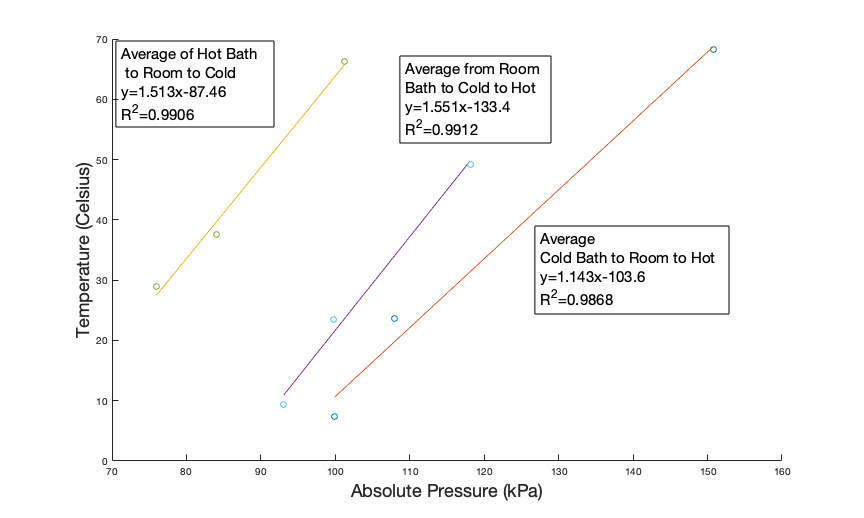
\includegraphics[width=16cm]{ex2.png}\\\textbf{Graph 2}: According from the information received from Appendix 1, the multiple trial graphs were created. The independent value $x$ is the absolute pressure measured in kilopascal, the dependent value $y$ is the temperature measured in Celsius. The purple graph contains an average slope of $1.551\pm 0.1463 \frac{\text{Celsius}}{kPa}$ with an average y-intercept of $-133.4\pm15.25 \text{ Celsius}$. The red graph contains an average slope of $1.143\pm 0.1321 \frac{\text{Celsius}}{kPa}$ with an average y-intercept of $-103.6\pm16.1 \text{ Celsius}$. The yellow graph contains an average slope of $1.513\pm 0.1472 \frac{\text{Celsius}}{kPa}$ with an average y-intercept of $-87.5\pm12.9 \text{ Celsius}$. Moreover, the $R^2$ value of these graphs are above $0.9868$ indicates that the data is above $98.6\%$ of the variation in the $y$ data is due to the variation in the $x$ data; giving a perfect slope of the alignment of the data. 
\end{center}
The average between all the absolute values and uncertainty calculations did not bring the experimental value closer to the theoretical value of $-273^\circ$ Celsius. The value obtained from the combination of the three processes was $-108\pm26^\circ$ Celsius. Unfortunately, the experimental error lies within an error percentage of $60\%$. That could be for many reasons: there were not enough data acquired with different tools, tools used might have been damaged and severely affecting the calculations considering that all the absolute zero values were under the theoretical value, the temperature fluctuates quickly, the acquisition of data was not the best. 

\section*{Discussion and Conclusion}
To conclude, the purpose of this experiment was to investigate the absolute zero at different types of states when the moles were constant and when moles were fluctuating in an ideal gas law formula.\\
When keeping the number of moles constant, the spherical apparatus went through different temperatures to get a linear trend between all the data points. The apparatus went from cold to warm to room-temperature water; therefore, affecting the data points. The linear trend acquired from this experiment was $y=2.7x-190$. Since the absolute pressure is on the independent axis $x$, the absolute zero is the y-intercept of the function; meaning, that the absolute pressure is equal to zero, which follows well with theory. Therefore, the absolute zero of the linear trend is $-190\pm11$ Celsius. Making the error percentage of $30\%$ due to several reasons. Statistically speaking, to have an accurate laboratory, there need to be many data points. The amount of data collected was not enough. By taking a look at graph 1, there is a total of seven data points that came into play with an $R^2$ value of 0.99, giving a perfect trend.  However, considering the equipment's faultiness, there could have been different apparatus' that could have been used to collect different amounts of data points. Considering that the apparatus goes from cold water to hot water to room-temperature water, the apparatus has not gone through the proper stages to collect practical data since the temperature from the previous water temperatures has affected the apparatus. Moreover, the equipment staff mentioned the faultiness of the equipment. Nonetheless, the data acquisition could have been wrong, considering that the temperature was forever fluctuating in a specific range of degrees. Accounting for both human errors and systematic errors coming from the machinery used. \\
Lastly, fluctuating the number of moles and setting the apparatus to different water temperatures provided an insight on the slopes from equations (2) and (1). The slopes found in the experimental graph (2) gave an insight into how many moles were in the sphere when the sphere was dumped into the water. When the sphere went from a hot bath to room-temperature water to cold water, the slope was $1.51 \frac{\tect{Celsius}}{kPa}$; given that the gas constant is $8.3 \frac{J}{mol\cdot k}$, and the volume of the sphere is $0.53$ litres—making the number of moles 0.043 mols. When the sphere went from room-temperature water to cold bath to hot water, the slope was $1.6 \frac{\tect{Celsius}}{kPa}$, making the number of moles $0.04$. Finally, from the cold bath to room-temperature to hot water, the slope was $1.1 \frac{\tect{Celsius}}{kPa}$, making 0.06 mols. Therefore, each different number of moles will result in a different slope as predicted. For different slopes, there will be different absolute zero values due to the y-intercept following the slope. Thus, the y-intercept for $0.043$ mols the absolute zero was at $-88\pm13$ Celsius; the absolute zero for $0.04$ was $-133\pm15$ Celsius; the y-intercept for $0.06$ mols was $-104\pm16$ Celsius. Unfortunately, the error percentage of all experimental absolute zero values compared to the $-273^\circ$ value is above $30\%$ error. Even with the average between all the values being $-108\pm26^\circ$ Celsius, it gives an error percentage of $60\%$. As mentioned previously, the error can be due to many factors. These factors may include both human errors, systematic errors from the machinery, and the number of moles in the system. A way to avoid such problems is to have at least 20 data points from five different apparatuses given a combination of 100 data points per segment of the experiment and done the average and standard deviation between all of them. However, due to a pandemic, it was impossible to redo the laboratory experiment, nor did the school had the luxury to supply multiple apparatuses. The theory did not get proven, but with shared knowledge and scientific exploration, $-273^\circ$ Celsius is the absolute zero. 

\newpage
\section*{Appendix}
Wagih, Ghobriel: Lab manual I: Introduction to Experimental Physics.
\begin{table}[h!]
\centering
 \begin{tabular}{||c c||} 
 \hline
 Absolute Pressure & Temperature \\ [0.5ex] 
 \hline\hline
     74.9 & 9.4  \\
     74.8 & 9.1  \\
     74.6 & 8.5  \\
     74.3 & 8.5  \\
     74.2 & 7.7  \\
     74.2 & 7.5  \\
     \vdots & \vdots 
 \end{tabular}
\end{table}
\\\small\textbf{Table1}: This table helped construct the first graph of the data anylisis. \\
\begin{center}
    \textbf{Appendix 1}: Data Points and Slopes Collected Trough Different Values of Moles and Temperature \\
    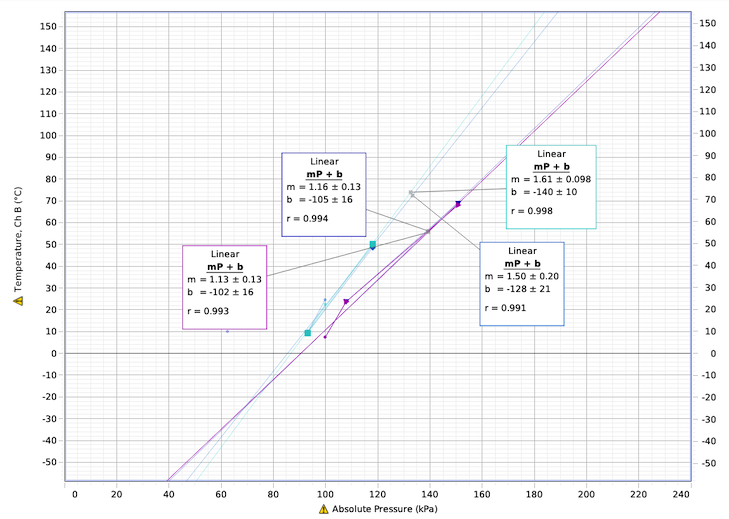
\includegraphics[width=15cm]{qwe.png}\\\textbf{Appendix 1}: From the raw data collected, the Capstone data was able to provide the slopes of the graph within three points. The independent value is the Absolute pressure and the dependent value is the temperature. 
\end{center}
Example of Calculations:\\
Dimensions of the apparatus sphere:
\[\text{Volume of sphere:} 35.66dm^3=32.66/61.024=0.53520151 L\]
Calculating Moles:
\[\text{Slope}=1.51\]\[\text{Volume}=0.54\]\[R=8.3145\]\[\frac{V}{n\cdot R}=\text{Slope}\]
\[n=\frac{V}{\text{Slope}\cdot n}=\frac{0.54}{1.51\cdot 8.3145}=0.0426289\]
The average between Absolute Zero:
\[\bar X= \frac{1}{n}\sum^n_{i\in\N}X_i=\frac{(-88)+(-104)+(-133)}{3}=-108 \%\]
Uncertainty for Absolute Zero:
 \[\frac{S}{-108}=\sqrt{\frac{S^2}{(-88)^2}+\frac{S^2}{-133}^2+\frac{S^2}{-104}}=\sqrt{\frac{13}^2{-88}^2+\frac{15^2}{(-133)^2}+\frac{16^2}{(-104)^2}}=-26.26^\circ\]
 Error Percentage between Experimental absolute zero and theoretical
 \[\frac{|theoretical-experimental|}{experimental}\cdot 100\% =\frac{|-273-(-108)}{-273}\cdot 100\%=60.44\%\]
 \newpage
 \begin{center}
 MatLab Code
     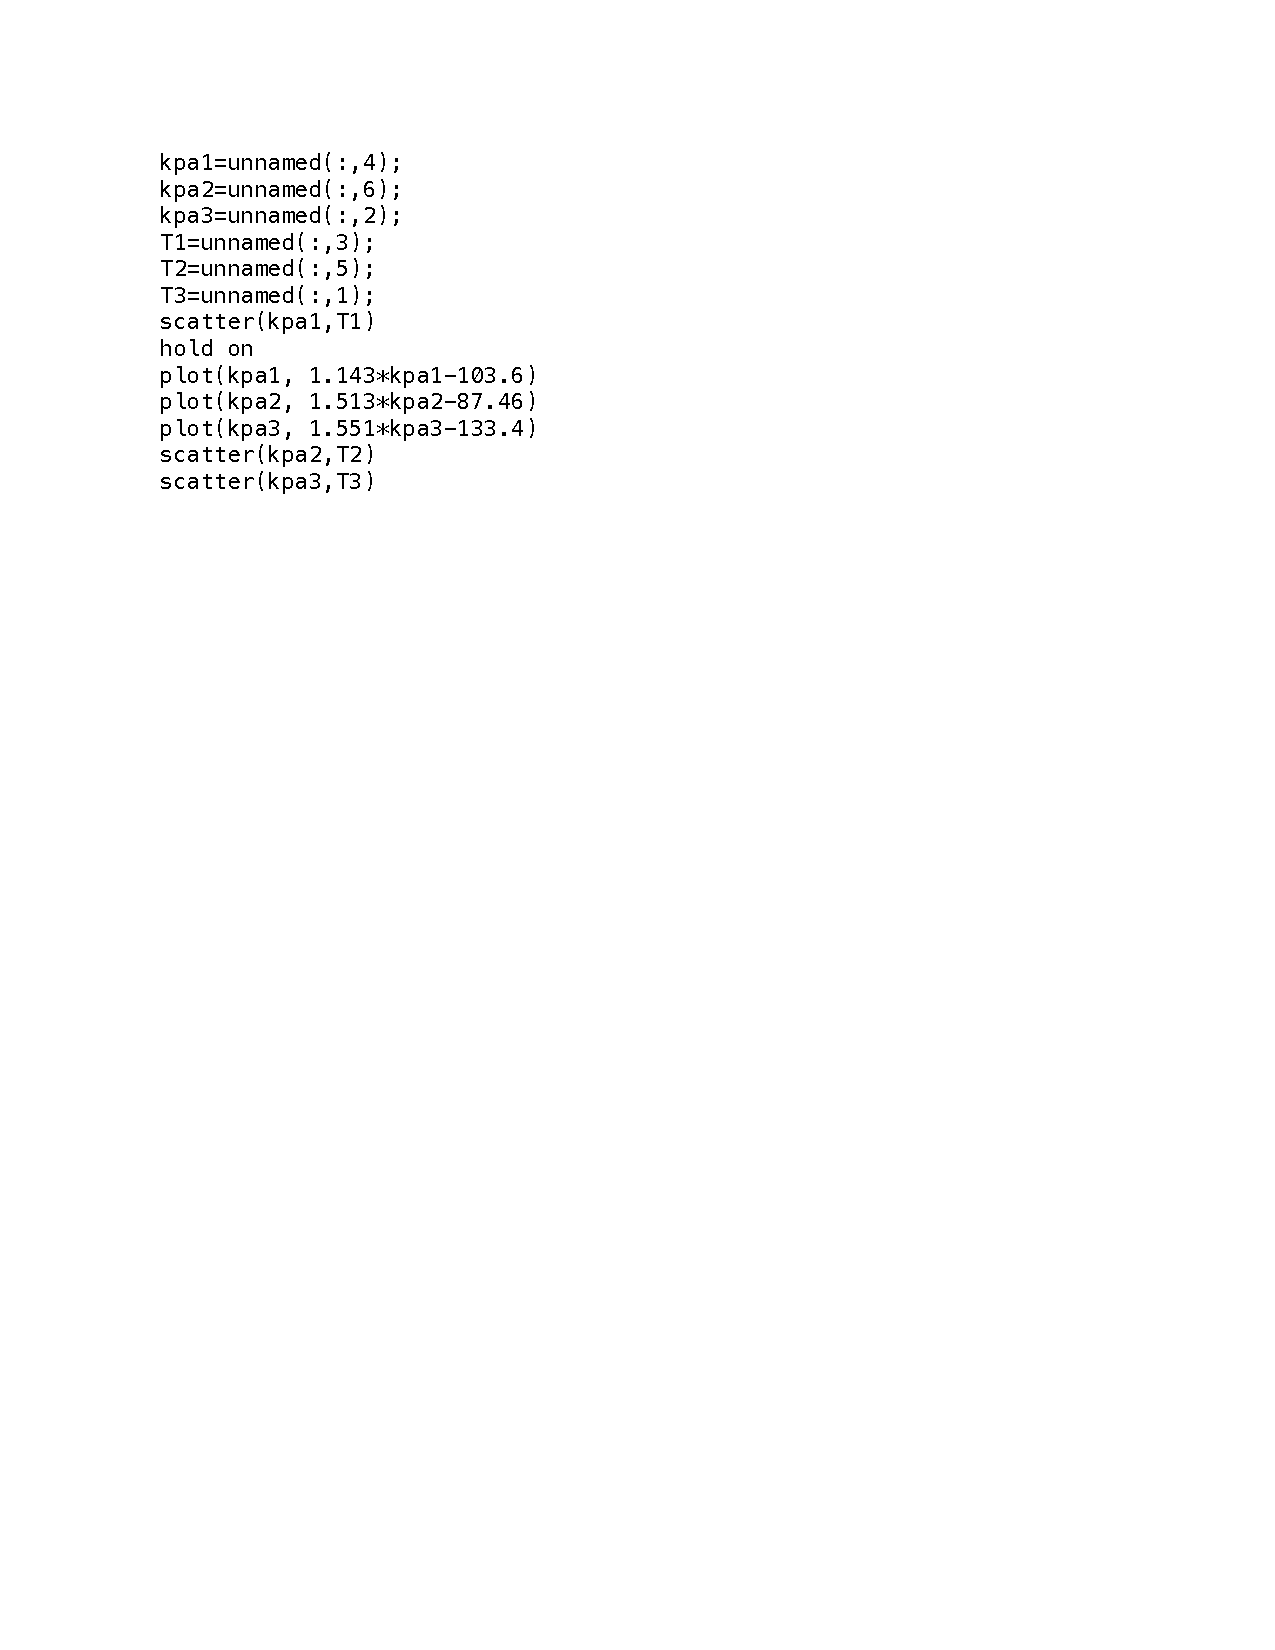
\includegraphics[width=16cm]{untitled.pdf}
 \end{center}

\end{document}